
\pdfminorversion=4 % for acroread
%\documentclass[aspectratio=169,t,xcolor={usenames,dvipsnames}]{beamer}
\documentclass[aspectratio=169,t,handout,xcolor={usenames,dvipsnames}]{beamer}
\usepackage{../beamerstyle}
\usepackage{dsfont}
\usepackage{bm}
\usepackage[english]{babel}
\usepackage[utf8]{inputenc}
\usepackage{graphicx}
\usepackage{algorithm}
\usepackage[ruled,vlined,algo2e,linesnumbered]{algorithm2e}
%\usepackage[boxed,vlined]{algorithm2e}
\usepackage{hyperref}
\usepackage{booktabs}
\usepackage{mathtools}

\usepackage{amsmath,amssymb}
\usepackage{listings}
\lstset{frame=lines,framesep=3pt,numbers=left,numberblanklines=false,basicstyle=\ttfamily\small}

\usepackage{subfig}
\usepackage{multicol}
%\usepackage{appendixnumberbeamer}
%
\usepackage{tcolorbox}

\usepackage{pgfplots}
\usepackage{tikz}
\usetikzlibrary{trees} 
\usetikzlibrary{shapes.geometric}
\usetikzlibrary{positioning,shapes,shadows,arrows,calc,mindmap}
\usetikzlibrary{positioning,fadings,through}
\usetikzlibrary{decorations.pathreplacing}
\usetikzlibrary{intersections}
\usetikzlibrary{positioning,fit,calc,shadows,backgrounds}
\pgfdeclarelayer{background}
\pgfdeclarelayer{foreground}
\pgfsetlayers{background,main,foreground}
\tikzstyle{activity}=[rectangle, draw=black, rounded corners, text centered, text width=8em]
\tikzstyle{data}=[rectangle, draw=black, text centered, text width=8em]
\tikzstyle{myarrow}=[->, thick, draw=black]

% Define the layers to draw the diagram
\pgfdeclarelayer{background}
\pgfdeclarelayer{foreground}
\pgfsetlayers{background,main,foreground}

%\usepackage{listings}
%\lstset{numbers=left,
%  showstringspaces=false,
%  frame={tb},
%  captionpos=b,
%  lineskip=0pt,
%  basicstyle=\ttfamily,
%%  extendedchars=true,
%  stepnumber=1,
%  numberstyle=\small,
%  xleftmargin=1em,
%  breaklines
%}

 
\definecolor{blue}{RGB}{0, 74, 153}

\usetheme{Boadilla}
%\useinnertheme{rectangles}
\usecolortheme{whale}
\setbeamercolor{alerted text}{fg=blue}
\useoutertheme{infolines}
\setbeamertemplate{navigation symbols}{\vspace{-5pt}} % to lower the logo
\setbeamercolor{date in head/foot}{bg=white} % blue
\setbeamercolor{date in head/foot}{fg=white}
\setbeamercolor{author  in head/foot}{bg=white} %blue
\setbeamercolor{title in head/foot}{bg=white} % blue
\setbeamercolor{title}{fg=white, bg=blue}
\setbeamercolor{block title}{fg=white,bg=blue}
\setbeamercolor{block body}{bg=blue!10}
\setbeamercolor{frametitle}{fg=white, bg=blue}
\setbeamercovered{invisible}

\makeatletter
\setbeamertemplate{footline}
{
  \leavevmode%
  \hbox{%
  \begin{beamercolorbox}[wd=.333333\paperwidth,ht=2.25ex,dp=1ex,center]{author in head/foot}%
%    \usebeamerfont{author in head/foot}\insertshortauthor
  \end{beamercolorbox}%
  \begin{beamercolorbox}[wd=.333333\paperwidth,ht=2.25ex,dp=1ex,center]{title in head/foot}%
    \usebeamerfont{title in head/foot}\insertshorttitle
  \end{beamercolorbox}%
  \begin{beamercolorbox}[wd=.333333\paperwidth,ht=2.25ex,dp=1ex,right]{date in head/foot}%
    \usebeamerfont{date in head/foot}\insertshortdate{}\hspace*{2em}
%    \insertframenumber\hspace*{2ex} 
  \end{beamercolorbox}}%
  \vskip0pt%
}
\makeatother

%\pgfdeclareimage[height=1.2cm]{automl}{images/logos/automl.png}
%\pgfdeclareimage[height=1.2cm]{freiburg}{images/logos/freiburg}

%\logo{\pgfuseimage{freiburg}}

\renewcommand{\comment}[1]{
	\noindent
	%\vspace{0.25cm}
	{\color{red}{\textbf{TODO:} #1}}
	%\vspace{0.25cm}
}
\newcommand{\notefh}[1]{\textcolor{red}{\textbf{FH:} #1}}
\renewcommand{\comment}[1]{}
\newcommand{\hide}[1]{}
\newcommand{\cemph}[2]{\emph{\textcolor{#1}{#2}}}

\newcommand{\lit}[1]{{\footnotesize\color{black!60}[#1]}}

\newcommand{\litw}[1]{{\footnotesize\color{blue!20}[#1]}}


\newcommand{\myframe}[2]{\begin{frame}[c]{#1}#2\end{frame}}
\newcommand{\myframetop}[2]{\begin{frame}{#1}#2\end{frame}}
\newcommand{\myit}[1]{\begin{itemize}#1\end{itemize}}
\newcommand{\myblock}[2]{\begin{block}{#1}#2\end{block}}


\newcommand{\votepurple}[1]{\textcolor{Purple}{$\bigstar$}}
\newcommand{\voteyellow}[1]{\textcolor{Goldenrod}{$\bigstar$}}
\newcommand{\voteblue}[1]{\textcolor{RoyalBlue}{$\bigstar$}}
\newcommand{\votepink}[1]{\textcolor{Pink}{$\bigstar$}}

\newcommand{\diff}{\mathop{}\!\mathrm{d}}
\newcommand{\refstyle}[1]{{\small{\textcolor{gray}{#1}}}}
\newcommand{\hands}[0]{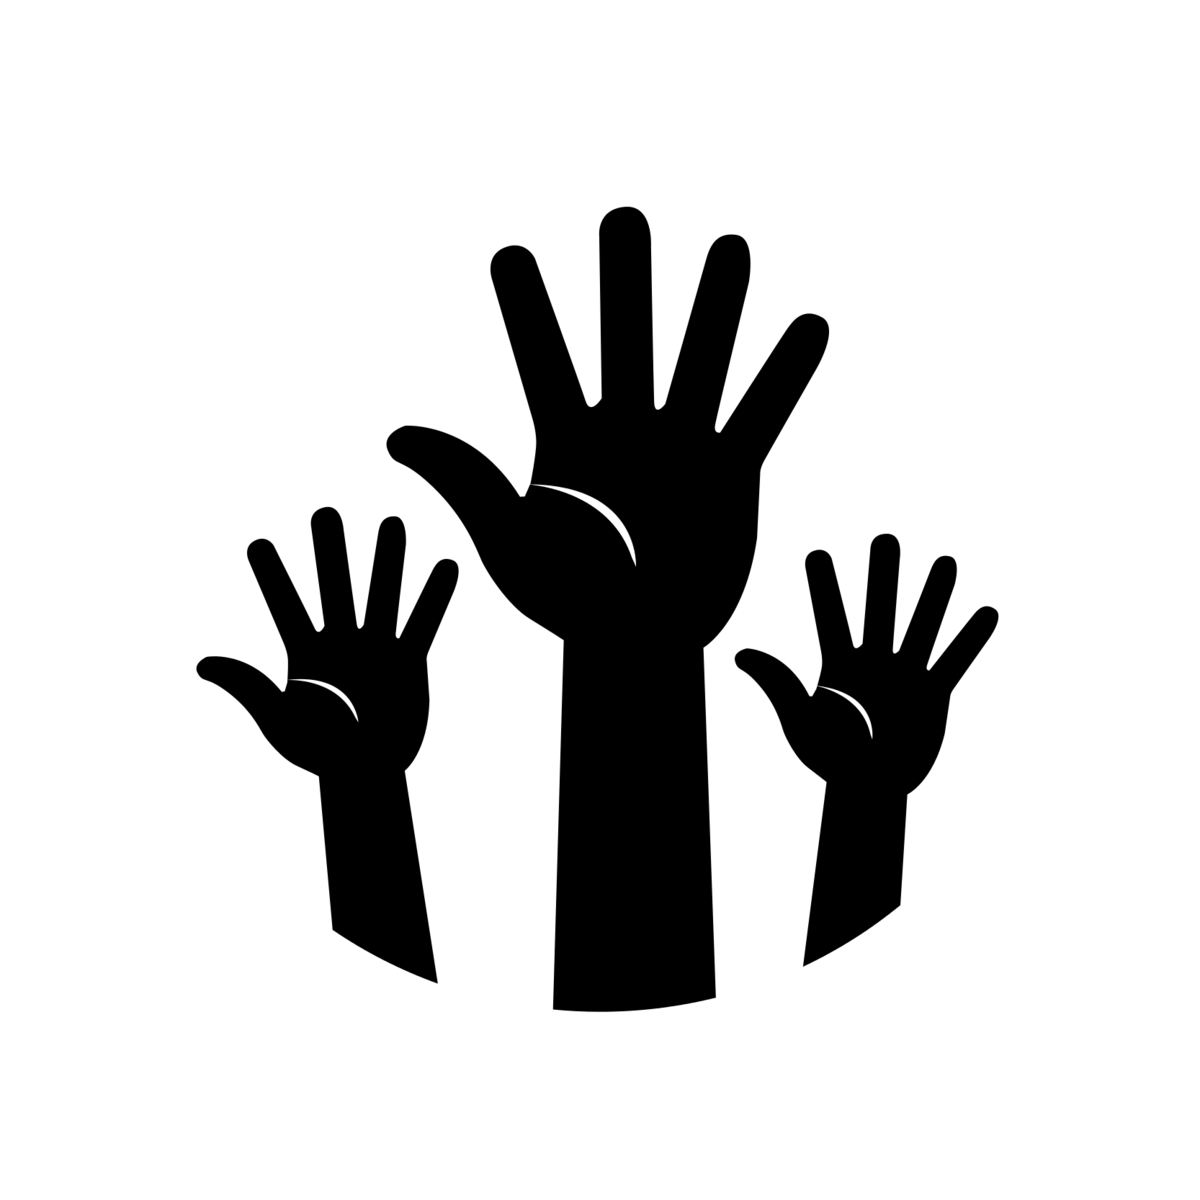
\includegraphics[height=1.5em]{images/hands}}
\newcommand{\transpose}[0]{{\textrm{\tiny{\sf{T}}}}}
\newcommand{\norm}{{\mathcal{N}}}
\newcommand{\cutoff}[0]{\kappa}
\newcommand{\instD}[0]{\dataset}
\newcommand{\insts}[0]{\mathcal{I}}
\newcommand{\inst}[0]{i}
\newcommand{\instI}[1]{i^{(#1)}}

% Iteration specific instance of variable/function/anything
% Introduced in the BO section, but moved up here to make it available within other macros
\newcommand{\iter}[2][\bocount]{{#2}^{(#1)}}

%--------HPO parameter macros-----------

% Parameter Configuration Space
\newcommand{\pcs}[0]{\pmb{\Lambda}}

% ???
\newcommand{\bx}[0]{\conf}

% Parameter Configuration
\newcommand{\conf}[0]{\pmb{\lambda}}

% Final Configuration
\newcommand{\finconf}[0]{\pmb{\hat{\lambda}}}

% Configuration corresponding to a given iteration -- better use \iter!
\newcommand{\confI}[1]{{\conf}^{(#1)}}

% Default Configuration
\newcommand{\defconf}[0]{{\conf}_{\text{def}}}

% Incumbent Configuration
\newcommand{\incumbent}[1][\bocount]{\iter[#1]{\finconf}}

% Optimal Configuration
\newcommand{\optconf}[0]{{\conf}^*}

% Configuration Space
\newcommand{\confs}[0]{\pcs}

%----------------------------------------

%\newcommand{\vlambda}[0]{\bm{\lambda}}
%\newcommand{\vLambda}[0]{\bm{\Lambda}}
\newcommand{\dataset}[0]{\mathcal{D}}
\newcommand{\datasets}[0]{\mathbf{D}}
\newcommand{\loss}[0]{L}
\newcommand{\risk}{\mathcal{R}}
\newcommand{\riske}{\mathcal{R}_{\text{emp}}}
\newcommand{\cost}[0]{c}
\newcommand{\costI}[1]{c^{(#1)}}

% Gaussian Process
\newcommand{\gp}{\mathcal{G}}
% Family of Objective Functions
\newcommand{\objF}{F}

%---------------BO Macros------------------

% BO loop counter
\newcommand{\bocount}{t}
% BO loop counter max, the counter runs from 1 to this value
\newcommand{\bobudget}{T}
% BO loop observation
\newcommand{\obs}[1][\conf]{\cost({#1})}
% BO loop observation space
\newcommand{\obsspace}{\mathcal{Y}}
% BO loop next observation
\newcommand{\bonextobs}{\obs[\iter{\conf}]}
% Acquisition Function, no args
\newcommand{\acq}{u}
% Standard Normal PDF
\newcommand{\pdf}{\phi}
% Standard Normal CDF
\newcommand{\cdf}{\Phi}
% Mean
\newcommand{\mean}{\mu}
% Standard Deviation
\newcommand{\stddev}{\sigma}
% Variance
\newcommand{\variance}{\sigma^2}
% Noise
\newcommand{\noise}{\nu}
% BO loop next selected sample
\newcommand{\bonextsample}{\confI{\bocount}}

% Single hyperparameter
\newcommand{\hyperparam}{\lambda}

% Single hyperparameter within a hyperparameter configuration
\newcommand{\hyperparami}[1][i]{{\hyperparam}_#1}

% Full definition of final configuration
\newcommand{\finconffull}{\incumbent[\bobudget]}

% Dataset
\newcommand{\datasetHPO}{{\dataset}_{HPO}}

% Dataset definition
\newcommand{\datasetHPOdef}{{\langle \bonextsample,\,\bonextobs \rangle}_{\bocount=1}^{\bobudget}}

% Double Display Fraction, forces large displays for everything in numerator and denominator
\newcommand\ddfrac[2]{\frac{\displaystyle #1}{\displaystyle #2}}

% Conditional Probability "Given That" Relation, source:https://tex.stackexchange.com/a/141685/205886
\newcommand\given[1][]{\:#1\vert\:}

% Expectation as a math operator
\DeclareMathOperator*{\E}{\mathbb{E}}

% Citation 
\newcommand{\source}[1]{
    \begin{flushright}
    	Source: \lit{#1}
    \end{flushright}
}
%-------------------------------------------

%Real numbers set
\newcommand{\realnum}{\mathbb{R}}
%Configuration space - do not use
%\newcommand{\configspace}{\Theta}
%Instances - do not use
%\newcommand{\instances}{\mathcal{I}}
%Expected value
\newcommand{\expectation}{\mathbb{E}}
%Kernel
\newcommand{\kernel}{\kappa}
%Constraint function
\newcommand{\constraintf}{c}
%Normal distribution
\newcommand{\normaldist}{\mathcal{N}}

% \renewcommand{\vec}[1]{\mathbf{#1}}
\newcommand{\hist}[0]{\dataset_{\text{Hist}}}
\newcommand{\param}[0]{p}
\newcommand{\algo}[0]{\mathcal{A}}
\newcommand{\algos}[0]{\mathbf{A}}
%\newcommand{\nn}[0]{N}
\newcommand{\feats}[0]{\mathcal{X}_{\text{meta}}}
\newcommand{\feat}[0]{\x_{\text{meta}}}
%\newcommand{\cluster}[0]{\vec{h}}
%\newcommand{\clusters}[0]{\vec{H}}
\newcommand{\perf}[0]{\mathbb{R}}
%\newcommand{\surro}[0]{\mathcal{S}}
\newcommand{\surro}[0]{\hat{\cost}}
\newcommand{\func}[0]{f}
\newcommand{\epm}[0]{\surro}
\newcommand{\portfolio}[0]{\mathbf{P}}
\newcommand{\schedule}[0]{\mathcal{S}}

% Machine Learning
\newcommand{\mdata}[0]{\dataset_{\text{meta}}}
\newcommand{\datasettrain}[0]{\dataset_{\text{train}}}
\newcommand{\datasetval}[0]{\dataset_{\text{val}}}
\newcommand{\datasettest}[0]{\dataset_{\text{test}}}
\newcommand{\x}[0]{\mathbf{x}}
\newcommand{\y}[0]{y}
\newcommand{\xI}[1]{\mathbf{x}^{(#1)}}
\newcommand{\yI}[1]{y^{(#1)}}
\newcommand{\fx}{f(\mathbf{x})}  % f(x), continuous prediction function
\newcommand{\Hspace}{\mathcal{H}} % hypothesis space where f is from
\newcommand{\fh}{\hat{f}}       % f hat, estimated prediction function

% Deep Learning
\newcommand{\weights}[0]{\theta}
\newcommand{\metaweights}[0]{\phi}


% reinforcement learning
\newcommand{\policies}[0]{\mathbf{\Pi}}
\newcommand{\policy}[0]{\pi}
\newcommand{\actionRL}[0]{a}
\newcommand{\stateRL}[0]{s}
\newcommand{\statesRL}[0]{\mathcal{S}}
\newcommand{\rewardRL}[0]{r}
\newcommand{\rewardfuncRL}[0]{\mathcal{R}}

\RestyleAlgo{algoruled}
\DontPrintSemicolon
\LinesNumbered
\SetAlgoVlined
\SetFuncSty{textsc}

\SetKwInOut{Input}{Input}
\SetKwInOut{Output}{Output}
\SetKw{Return}{return}

%\newcommand{\changed}[1]{{\color{red}#1}}

%\newcommand{\citeN}[1]{\citeauthor{#1}~(\citeyear{#1})}

\renewcommand{\vec}[1]{\mathbf{#1}}
\DeclareMathOperator*{\argmin}{arg\,min}
\DeclareMathOperator*{\argmax}{arg\,max}

%\newcommand{\aqme}{\textit{AQME}}
%\newcommand{\aslib}{\textit{ASlib}}
%\newcommand{\llama}{\textit{LLAMA}}
%\newcommand{\satzilla}{\textit{SATzilla}}
%\newcommand{\satzillaY}[1]{\textit{SATzilla'{#1}}}
%\newcommand{\snnap}{\textit{SNNAP}}
%\newcommand{\claspfolioTwo}{\textit{claspfolio~2}}
%\newcommand{\flexfolio}{\textit{FlexFolio}}
%\newcommand{\claspfolioOne}{\textit{claspfolio~1}}
%\newcommand{\isac}{\textit{ISAC}}
%\newcommand{\eisac}{\textit{EISAC}}
%\newcommand{\sss}{\textit{3S}}
%\newcommand{\sunny}{\textit{Sunny}}
%\newcommand{\ssspar}{\textit{3Spar}}
%\newcommand{\cshc}{\textit{CSHC}}
%\newcommand{\cshcpar}{\textit{CSHCpar}}
%\newcommand{\measp}{\textit{ME-ASP}}
%\newcommand{\aspeed}{\textit{aspeed}}
%\newcommand{\autofolio}{\textit{AutoFolio}}
%\newcommand{\cedalion}{\textit{Cedalion}}
\newcommand{\fanova}{\textit{fANOVA}}
\newcommand{\sbs}{\textit{SB}}
\newcommand{\oracle}{\textit{VBS}}

% like approaches
\newcommand{\claspfoliolike}[1]{\texttt{claspfolio-#1-like}}
\newcommand{\satzillalike}[1]{\texttt{SATzilla'#1-like}}
\newcommand{\isaclike}{\texttt{ISAC-like}}
\newcommand{\ssslike}{\texttt{3S-like}}
\newcommand{\measplike}{\texttt{ME-ASP-like}}

\newcommand{\irace}{\textit{I/F-race}}
\newcommand{\gga}{\textit{GGA}}
\newcommand{\smac}{\textit{SMAC}}
\newcommand{\paramils}{\textit{ParamILS}}
\newcommand{\spearmint}{\textit{Spearmint}}
\newcommand{\tpe}{\textit{TPE}}


\usepackage{pifont}
\newcommand{\itarrow}{\mbox{\Pisymbol{pzd}{229}}}
\newcommand{\ithook}{\mbox{\Pisymbol{pzd}{52}}}
\newcommand{\itcross}{\mbox{\Pisymbol{pzd}{56}}}
\newcommand{\ithand}{\mbox{\raisebox{-1pt}{\Pisymbol{pzd}{43}}}}

%\DeclareMathOperator*{\argmax}{arg\,max}

\newcommand{\ie}{{\it{}i.e.\/}}
\newcommand{\eg}{{\it{}e.g.\/}}
\newcommand{\cf}{{\it{}cf.\/}}
\newcommand{\wrt}{\mbox{w.r.t.}}
\newcommand{\vs}{{\it{}vs\/}}
\newcommand{\vsp}{{\it{}vs\/}}
\newcommand{\etc}{{\copyedit{etc.}}}
\newcommand{\etal}{{\it{}et al.\/}}

\newcommand{\pscProc}{{\bf procedure}}
\newcommand{\pscBegin}{{\bf begin}}
\newcommand{\pscEnd}{{\bf end}}
\newcommand{\pscEndIf}{{\bf endif}}
\newcommand{\pscFor}{{\bf for}}
\newcommand{\pscEach}{{\bf each}}
\newcommand{\pscThen}{{\bf then}}
\newcommand{\pscElse}{{\bf else}}
\newcommand{\pscWhile}{{\bf while}}
\newcommand{\pscIf}{{\bf if}}
\newcommand{\pscRepeat}{{\bf repeat}}
\newcommand{\pscUntil}{{\bf until}}
\newcommand{\pscWithProb}{{\bf with probability}}
\newcommand{\pscOtherwise}{{\bf otherwise}}
\newcommand{\pscDo}{{\bf do}}
\newcommand{\pscTo}{{\bf to}}
\newcommand{\pscOr}{{\bf or}}
\newcommand{\pscAnd}{{\bf and}}
\newcommand{\pscNot}{{\bf not}}
\newcommand{\pscFalse}{{\bf false}}
\newcommand{\pscEachElOf}{{\bf each element of}}
\newcommand{\pscReturn}{{\bf return}}

%\newcommand{\param}[1]{{\sl{}#1}}
\newcommand{\var}[1]{{\it{}#1}}
\newcommand{\cond}[1]{{\sf{}#1}}
%\newcommand{\state}[1]{{\sf{}#1}}
%\newcommand{\func}[1]{{\sl{}#1}}
\newcommand{\set}[1]{{\Bbb #1}}
%\newcommand{\inst}[1]{{\tt{}#1}}
\newcommand{\myurl}[1]{{\small\sf #1}}

\newcommand{\Nats}{{\Bbb N}}
\newcommand{\Reals}{{\Bbb R}}
\newcommand{\extset}[2]{\{#1 \; | \; #2\}}

\newcommand{\vbar}{$\,\;|$\hspace*{-1em}\raisebox{-0.3mm}{$\,\;\;|$}}
\newcommand{\vendbar}{\raisebox{+0.4mm}{$\,\;|$}}
\newcommand{\vend}{$\,\:\lfloor$}


\newcommand{\goleft}[2][.7]{\parbox[t]{#1\linewidth}{\strut\raggedright #2\strut}}
\newcommand{\rightimage}[2][.3]{\mbox{}\hfill\raisebox{1em-\height}[0pt][0pt]{\includegraphics[width=#1\linewidth]{#2}}\vspace*{-\baselineskip}}





\newcommand{\a}[0]{\mathbf{a}}
\newcommand{\y}[0]{\mathbf{y}}
\newcommand{\q}[0]{\mathbf{q}}
\newcommand{\Xspace}[0]{\mathcal{X}}
\usepackage[ruled,vlined]{algorithm2e}
\usepackage{algorithm}
\usepackage{algorithmic}
\title[AutoML: Overview]{Multi-criteria Optimization}
\subtitle{Evolutionary Approaches}
%TODO: change authors!
\author[Bernd Bischl]{Bernd Bischl \and Frank Hutter \and Lars Kotthoff \and \underline{Marius Lindauer}}
\institute{}
\date{}



% \AtBeginSection[] % Do nothing for \section*
% {
%   \begin{frame}{Outline}
%     \bigskip
%     \vfill
%     \tableofcontents[currentsection]
%   \end{frame}
% }

\begin{document}

	\maketitle




\begin{frame}[allowframebreaks]{A-posteriori methods and evolutionary algorithms}

Evolutionary algorithms return as a solution a \textbf{population} of solution candidates. Evolutionary multi-objective (EMO) algorithms aim to provide a set of solution candidates that corresponds to the Pareto set \enquote{as well as possible}.

\vspace*{-0.4cm}

\begin{center}
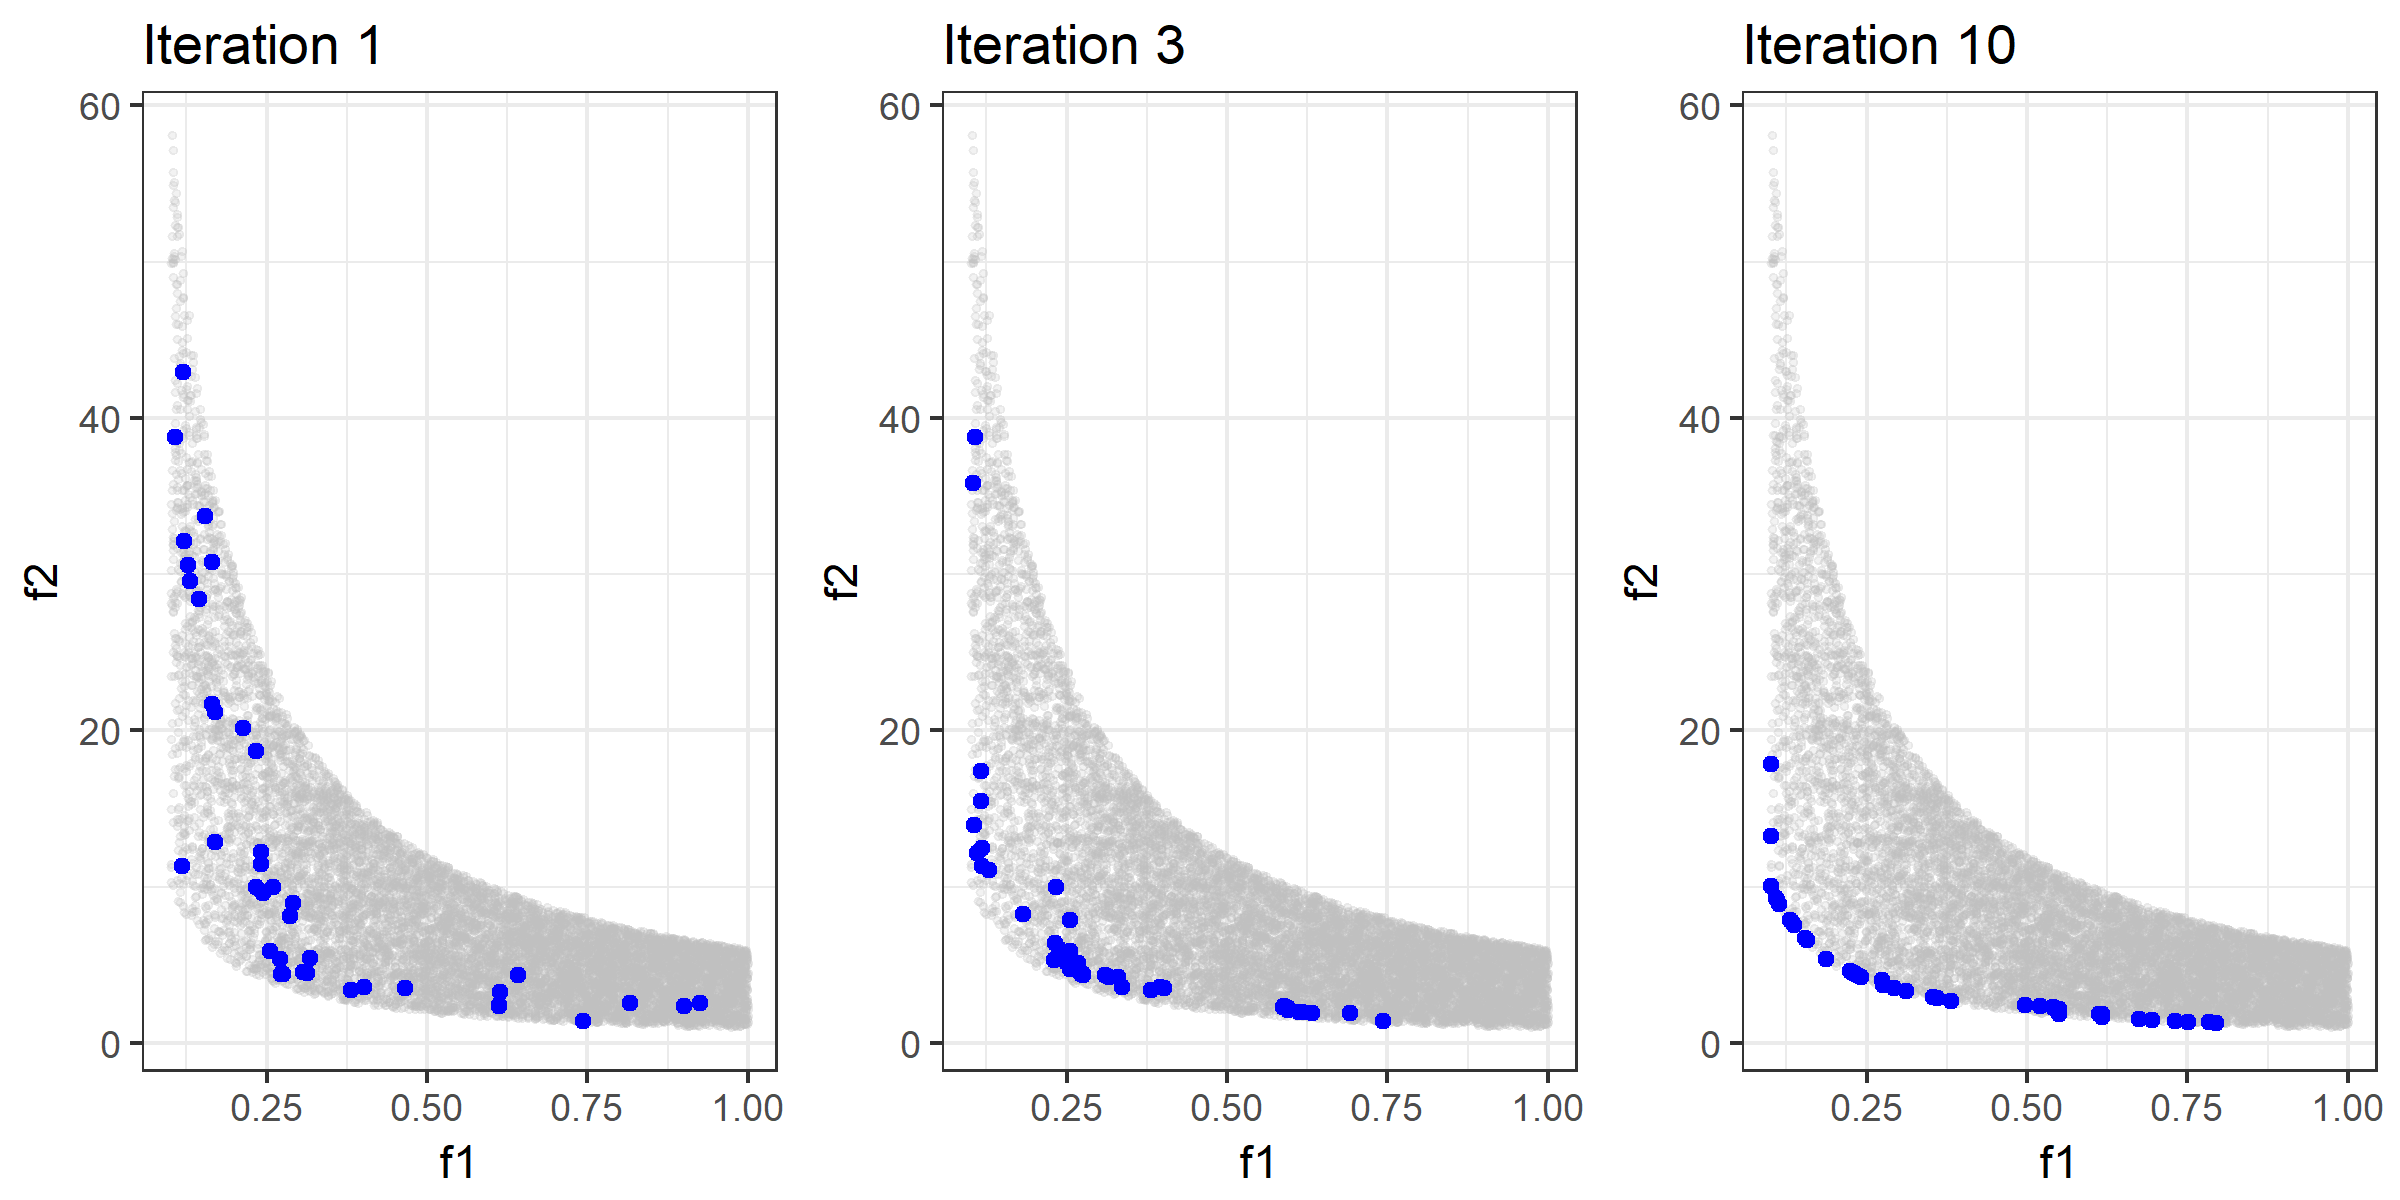
\includegraphics[width = 0.7\linewidth]{images/EA-steps.png}
\end{center}

\vspace*{-0.4cm}

\begin{footnotesize}
Image of the function (grey) and target function values $(f_1(\x), f_2(\x))$ for $\x \in \mathcal{P}_i, i = 1, 3, 10$.
\end{footnotesize}

\framebreak

\begin{algorithm}[H]
  \begin{center}
  \caption{Evolutionary algorithm}
    \begin{algorithmic}[1]
    \State Initialize and rate population $P_0 \subset \Xspace$ with $|\mathcal{P}| = \mu$
    \State $t \leftarrow 0$
      \Repeat
        \State Variation: generate offspring $Q_t$ with $|Q_t| = \lambda$
        \State Rate fitness of offspring
        \State Selection: select survivors $P_{t + 1}$
 		\State $t \leftarrow t + 1$
      \Until{Stop criterion fulfilled}
            \vspace*{-0.3cm}
    \end{algorithmic}
    \end{center}
\end{algorithm}

The population of solution candidates consists of $\x \in \Xspace$.

\end{frame}


\begin{frame}[allowframebreaks]{Objectives of an evolutionary strategy}

The aim is to select the evolution strategy in such a way that the algorithm provides an approximation of the Pareto front, where

\begin{enumerate}
\item The individuals of the population (or the corresponding functional values in the target function space) \textbf{converge} to the Pareto front.
\item The individuals of the population provide a \textbf{diverse} as possible approximation of the Pareto front.
\end{enumerate}

\vspace*{-0.3cm}

\begin{center}
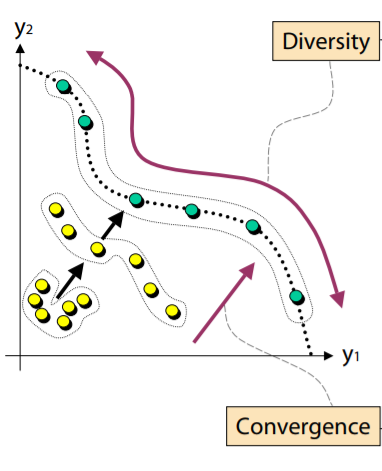
\includegraphics[width = 0.2\linewidth]{images/EMO_goals.png}
\end{center}

\vspace*{-0.5cm}

\begin{footnotesize}
\textbf{Caution}: in this graphic the objective function values are exceptionally \textbf{maximized}.
\end{footnotesize}

\end{frame}

\begin{frame}[allowframebreaks]{NSGA-II}

The \textbf{non-dominated sorting genetic algorithm (NSGA-II)} was published by K. Deb in 2002.

\begin{itemize}
\item The NSGA-II follows a $(\mu + \lambda)$ strategy
\item All previously discussed strategies can be used as a variation strategy; the original paper uses polynomial mutation and simulated binary crossover.
\item The selection strategy is based on
\begin{itemize}
\item \textbf{Non-dominated sorting}
\item \textbf{Crowding distance assignment}
\end{itemize}
\end{itemize}

\end{frame}

\begin{frame}[allowframebreaks]{NSGA-II: non-dominated sorting}

% \begin{center}
% 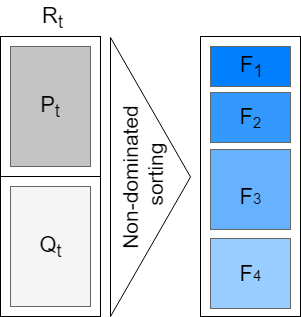
\includegraphics[width = 0.5\linewidth]{images/NSGA2_1.png}
% \end{center}

% \framebreak

\begin{footnotesize}
We subdivide $R_t = P_t \cup Q_t$ into fronts $F_1, F_2, F_3, ...$ such that

\begin{itemize}
\item the points in the fronts are equivalent to each other, and
\item that any point $\x \in F_1$ dominates any point from $F_2, F_3, F_4...$; any point $\x \in F_2$ dominates all points from $F_3, F_4, ...$, etc. \\
We write $F_1 \prec F_2 \prec F_4 \prec ... $
\end{itemize}
\end{footnotesize}

\begin{center}
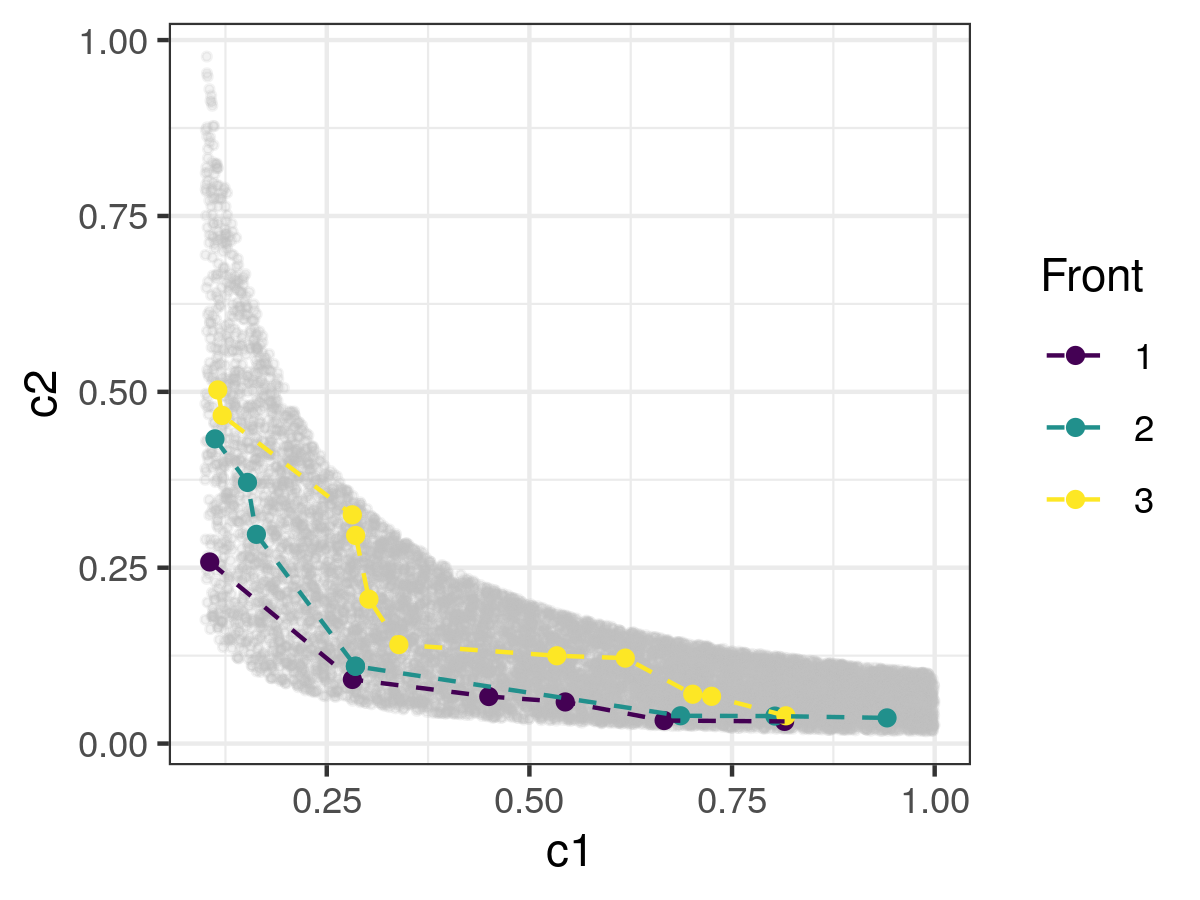
\includegraphics[width = 0.4\linewidth]{images/NSGA2_NDS.png}
\end{center}

\framebreak

Which individuals survive? We fill $\mu$ \enquote{places} one by one with $F_1, F_2, ...$ until a front can no longer \textbf{fully} survive (here: $F_3$).

\begin{center}
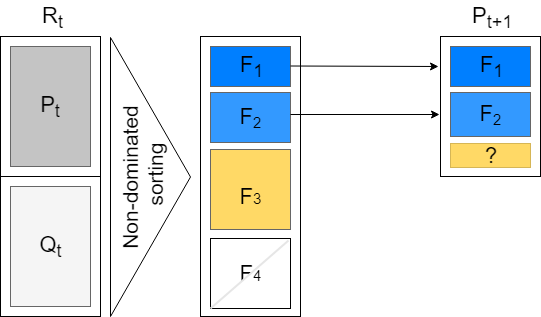
\includegraphics[width = 0.45\linewidth]{images/NSGA2_2.png}
\end{center}

Which individuals survive from $F_3$? $\to$ \textbf{crowding sort}

\end{frame}

\begin{frame}[allowframebreaks]{NSGA-II: crowding sort}

\textbf{Idea:} add a \enquote{good} representative of the front $F_3$ if possible.

\begin{center}
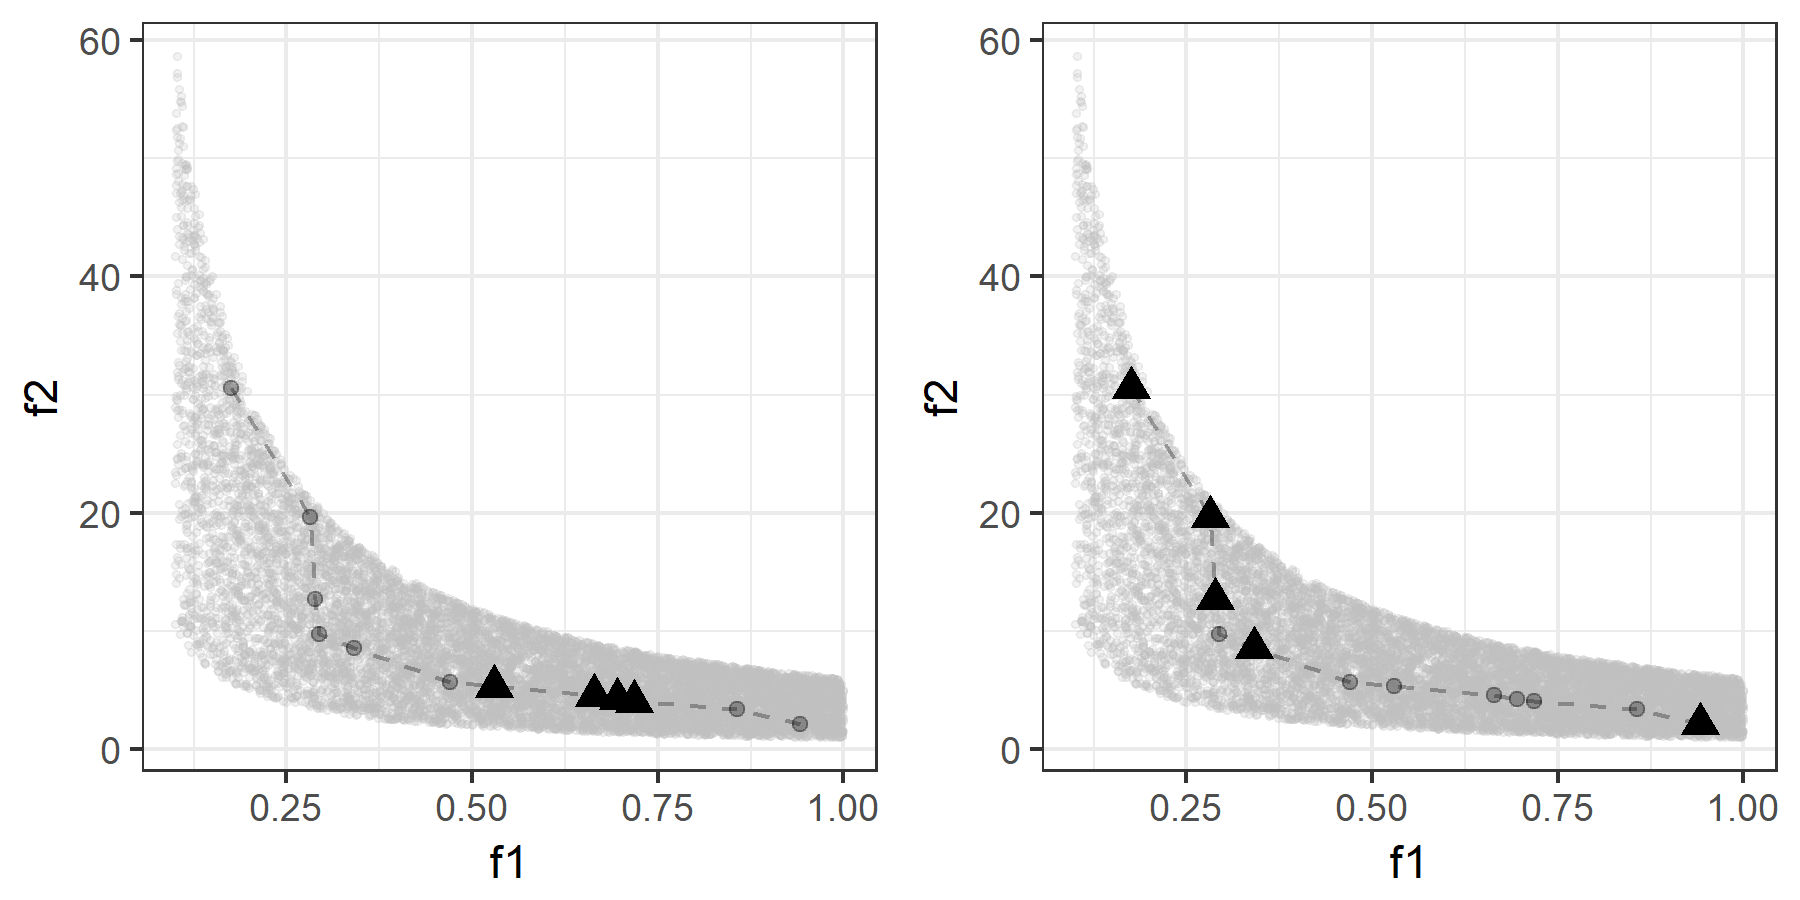
\includegraphics[height = 0.5\textheight]{images/NSGA2_CS1.png}
\end{center}

\begin{footnotesize}
The points on the left (marked by a triangle) do not represent the front very well because they are very close together. The front is better represented by the points on the right plot.
\end{footnotesize}

\framebreak

\textbf{Crowding sort} sorts the individuals based on their crowding distance:

\begin{itemize}
\item The crowding distance describes the solution density by one point.
\item It is calculated from the mean distance to the nearest neighbors around a point in the target function space.
\item The crowding distance is greater when the neighbors are very far away.
\item The maximum crowding distance is assigned to the boundary points so that they are always selected.
\end{itemize}

\begin{center}
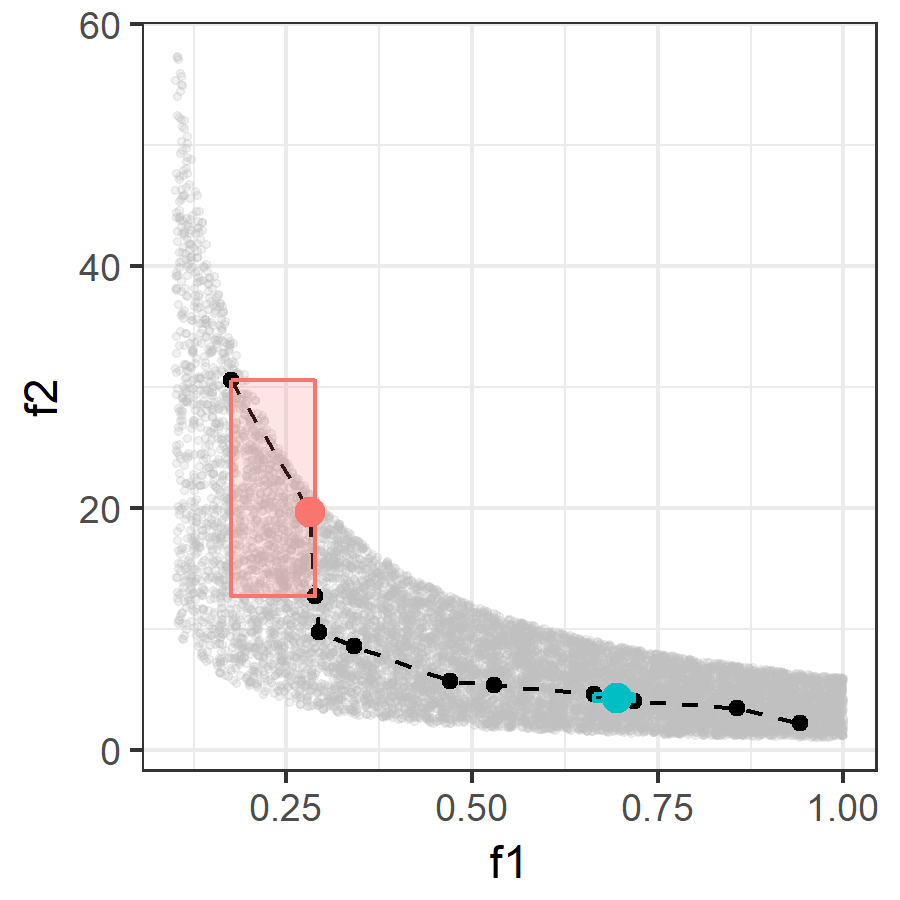
\includegraphics[width = 0.4\linewidth]{images/NSGA2_CS2.png}
\end{center}

\begin{footnotesize}
One point with high crowding distance (red) and one point with very small crowding distance (blue).
\end{footnotesize}

\framebreak

\begin{algorithm}[H]

  \begin{center}
  \caption{NSGA-II}
    \begin{algorithmic}[1]
   	\begin{footnotesize}
    \State Initialize population $P_0$, $t \leftarrow 0$
    \State $F_1, F_2, F_3, ... \leftarrow \texttt{nondominated-sort}(P_0)$
    \State Generate $Q_0$ by binary tournament selection, recombination and mutation
      \Repeat
        \State $F_1, F_2, F_3, ... \leftarrow \texttt{nondominated-sort}(P_t \cup Q_t)$
        \State $i \leftarrow 1$
        \While{$|P_{t + 1} \cup F_i| < \mu$}
        	\State $P_{t + 1} = P_{t + 1} \cup F_i$
        	\State $i \leftarrow i + 1$
    	\EndWhile
        \State $\tilde F_i = (\x_1, \x_2, ..., \x_k)= \texttt{SortByCrowdingDistance}(F_i)$
        \While {$P_{t + 1} < \mu$}
        	\State $P_{t + 1} = P_{t + 1} \cup \x_j$
        	\State $j \leftarrow j + 1$
        \EndWhile
        \State Generate $Q_{t + 1}$ by binary tournament selection, recombination and mutation
      \Until{Stop criterion fulfilled}
      \vspace*{-0.3cm}
      \end{footnotesize}
    \end{algorithmic}
    \end{center}
\end{algorithm}

\end{frame}

% \begin{frame}[allowframebreaks]{SPEA-2}

% Ebenso im Jahr 2002 wurde der \textbf{Strength Pareto EA} (SPEA-2) von Zitzler et al. veröffentlicht.

% \lz

% \begin{itemize}
% \item Neben der aktuellen Population $P_t$ gibt es auch ein sogenanntes Archiv $A_t$, das lediglich zur Bewertung der aktuellen Population dient.

% \begin{images}
% 	\centering
% 	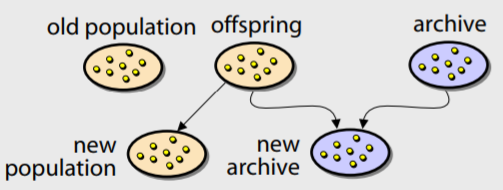
\includegraphics[width=0.6\linewidth]{images/SPEA-archive}
% \end{images}

% \framebreak

% \item Die Bewertung (und damit auch die Selektion) eines Individuums erfolgt anhand von

% $$
% \text{fitness}(x) = \text{raw}(x) + \text{density}(x).
% $$

% Hierbei ist

% \begin{itemize}
% \item $\text{raw}(x)$ die \enquote{Grundfitness} (bzgl. Population und Archiv)
% \vspace*{-0.2cm}
% $$
% \text{raw}(x) = |\{y \in P_t: f(x) \prec f(y)\}| + |\{y \in A_t: f(x) \prec f(y)\}|,
% $$

% \item $\text{density}(x)$ die Dichte des Punktes
% $$
% \text{density}(x) = \frac{1}{\sigma^{(k)}(x) + 2},
% $$
% ($\sigma^{(k)}$ bezeichne den Abstand zum $k$-nächsten Nachbarn).
% \end{itemize}
% \end{itemize}

% \framebreak

% \begin{algorithm}[H]
% \begin{footnotesize}
%   \begin{center}
%   \caption{SPEA-2}
%     \begin{algorithmic}[1]
%     \State Initialisiere Population $P_0$, $|P_0| = \lambda$ und ein leeres Archiv $A_0, |A_0| = \gamma$
%       \Repeat
%         \State Berechne Fitness der Individuen in $P_t$ und $A_t$ anhand der oben definierten Fitnessfunktion
%         \State Fülle $A_{t+1}$ auf mit nichtdominierten Individuen aus $P_t \cup A_t$ $^{(*)}$
%         \State Fülle \enquote{mating pool} durch binäre Turnierselektion mit Zurücklegen auf $A_{t + 1}$
%         \State Generiere $P_{t + 1}$ durch Rekombination und Mutation
%       \Until{Stoppkriterium erfüllt}
%       \State Gib $A_t$ zurück
%     \end{algorithmic}
%     \end{center}
% \end{footnotesize}
% \end{algorithm}

% \vfill
% \begin{footnotesize}
% $^{(*)}$ Wenn $|A_{t + 1}| > \gamma$, dann entferne solange Individuen mit kleinster Distanz zum Nachbarn, bis $|A_{t + 1}| = \gamma$. Sollte $|A_{t + 1}| < \gamma$, füge die besten dominierten Individuen aus $P_t \cup A_t$ hinzu.
% \end{footnotesize}

% \end{frame}


\begin{frame}[allowframebreaks]{Selection criteria: contribution to the hypervolume}

\begin{itemize}
\item The SMS-EMOA (S-Metric-Selection-EMOA) evaluates the fitness of an individual $\x \in \mathcal{P} \subset \Xspace$ based on its contribution to the dominated hypervolume (S-Metric):
$$
\Delta s(\x, \mathcal{P}) = S(\mathcal{P}, R) - S(\mathcal{P} \setminus \{ \x\}, R).
$$
\end{itemize}
% \framebreak

% \textbf{Berechnung des Hypervolumens im 2 dimensionalen Fall:}
% \begin{enumerate}
% \item Sortiere die Zielfunktionsvektoren bzgl. eines Kriteriums (z.B. aufsteigend bzgl. $f_1$)\\
% $\Rightarrow$ Da Pareto-Front (kein Punkt dominiert anderen): Punkte sind bzgl. $f_2$ absteigend sortiert .
% \item Für das $j$-te Individuum $a^{(j)}, j\in \{2,..., |F_{\nu}|\}$ in der sortierten Sequenz der Front $F_{\nu}$ berechnet sich der Hypervolumensbeitrag als:
% \medskip

% $$
% \Delta s(\y^{(j)}, F_{\nu}) = (y_{1}^{(j+1)} - y_{1}^{(j)}) (y_{2}^{(j-1)} - y_{2}^{(j)})
% $$
% \end{enumerate}

\framebreak

\begin{center}
Hypervolume contribution in a 2-dimensional objective space:\\
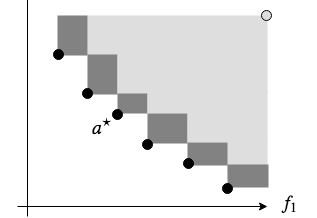
\includegraphics[width = 0.4\textwidth]{images/hypervolumenbeitrag.png}
\end{center}

\footnotesize
\vspace*{-0.5cm}
\begin{itemize}
% \item Links: Punkte entsprechen Werten der Individuen in 2-dimensionalem Zielraum.
% \item Links: Punkte ohne Füllung zeigen dominierte Lösungen. Gelbe Fläche zeigt Bereich in dem dominierende Lösungen liegen.
\item Dark rectangles correspond to the hypervolume contribution of the black dots.
\item Grey point is the so-called reference point and limits the space.
\item The hypervolume contribution thus corresponds to the size of the space that is dominated only by the individual $\bm{a}$, and not to any other of the space.
\item $a^\star$ has lowest S-metric contribution .
\end{itemize}
\end{frame}

% \begin{frame}[allowframebreaks]{SMS-EMOA}
% \textbf{Motivation:}
% \begin{itemize}
% \item Pareto-Front bildet Menge von optimalen Parameterkonbinationen ab.
% \item Oft ist die Menge dieser Kombinationen noch sehr groß.
% \item In Praxis ist es meist nicht möglich alle Pareto-Effizienten Lösungen zu prüfen
% \end{itemize}
% $\Rightarrow$ SMS-EMOA soll möglichst guten Kompromiss zwischen Aufwand der Überprüfung der Paretoeffizienten Lösungen bei gleichzeitig umfassender Abdeckung möglicher Kompromisslösungen darstellen.
% \medskip

% $\Rightarrow$ SMS-EMOA ist einfach handhabbar und verzichtet auf Erstellung eines Archivs um den Aufwand zu reduzieren.
% \medskip

% $\Rightarrow$ Optimierung wird allein auf Grundlage der Population durchgeführt.

% \framebreak
% \end{frame}

\begin{frame}[allowframebreaks]{SMS-EMOA algorithm}

\vspace*{-0.5cm}

\begin{algorithm}[H]
  \begin{center}
  \caption{SMS-EMOA}
    \begin{algorithmic}[1]
    \begin{footnotesize}
    \State Generate start population $P_0$ of size $\mu$
    \State $t \leftarrow 0$
      \Repeat
        \State Generate \textbf{one} individual $\q \in \R^n$ by recombination and mutation of $\mathcal{P}_t$
        \State $\{F_{1},..., F_k\} \leftarrow \text{fast-dominated-sort}(P_{t}\cup \q)$
        \State $\bm{a}^\star \leftarrow \text{argmin}_{\bm{a} \in F_{k}}\Delta s(\bm{a}, F_{k})$
        \State $P_{t+1} \leftarrow (P_t \cup \{\q\}) \setminus\{\bm{a}^\star\}$
        \State $ t \leftarrow t+1$
      \Until{Termination criterion fulfilled}
    \end{footnotesize}
    \vspace*{-0.3cm}
    \end{algorithmic}
    \end{center}
\end{algorithm}

\vspace*{-0.6cm}
\footnotesize
\begin{itemize}
\item L5: the set of temporary $(\mu + 1)$ individuals is divided by \textbf{fast-dominated-sort} into $k$ fronts $F_{1},...,F_{k}$.
\item L6: determine individual $\bm{a}^\star \in F_{k}$ with smallest hypervolume contribution.
\item L7: the individual $\bm{a}^\star$ from the worst front with the smallest contribution to the dominated hypervolume does not survive.
\item The fitness of an individual is therefore primarily the rank of its associated front and secondarily its contribution to hypervolume.
\end{itemize}
\end{frame}


\end{frame}
\end{document}
